\begin{to_def}
    \textit{Оптически мутной} называют среду с $\langle n\rangle = \const$, но содержащую макроскопические неоднородности. В таких средах свет \textit{рассеивается в стороны}, иначе это явление называют \textit{эффектом Тиндаля}\footnote{
        Теоретически обоснованным Рэлеем.
    }.
\end{to_def}

В неоднородной неподвижной изотропной среде распространение света описывается уравнениями Максвелла
\begin{align*}
    &\rot \vc{H} = \frac{\varepsilon}{c} \frac{\partial \vc{E}}{\partial t}, &\div(\varepsilon \vc{E}) = 0, \\
    &\rot \vc{E} = - \frac{1}{c} \frac{\partial \vc{H}}{\partial t}, &\div \vc{H} = 0,
\end{align*}
где $\varepsilon \equiv \varepsilon(x, y, z)$. Выделим $\varepsilon = \varepsilon_0 + \delta \varepsilon$, где $\varepsilon_0 = \const$. 


Можем представить ЭМ поле в виде $\vc{E} = \vc{E}_0 + \vc{E}'$, $\vc{H} = \vc{H}_0 + \vc{H}'$, где $\vc{E}_0$, $\vc{H}_0$ удовлетворяют уравнениям Максвелла в однородной среде
\begin{align*}
    &\rot \vc{H}_0 = \frac{\varepsilon_0}{c} \frac{\partial \vc{E}_0}{\partial t}, &\div(\varepsilon_0 \vc{E}_0) = 0, \\
    &\rot \vc{E}_0 = - \frac{1}{c} \frac{\partial \vc{H}_0}{\partial t}, &\div \vc{H}_0 = 0.
\end{align*}
Принята номенклатура о том, что $\vc{A}_0$ -- \textit{падающая волна}, а $\vc{A}'$ -- поле \textit{рассеянного света}. 

Вычитая последние две группы уравнений друг из друга, находим
\begin{align*}
    &\rot \vc{H}' - \frac{\varepsilon_0}{c} \frac{\partial \vc{E}'}{\partial t} = \frac{\delta \varepsilon}{c} \frac{\partial \vc{E}}{\partial t},  
    &\div (\varepsilon_0 \vc{E}') = - \div(\delta \varepsilon \, \vc{E}), \\
    &\rot \vc{E}' - \frac{1}{c}\frac{\partial \vc{H}'}{\partial t} = 0, 
    &\div \vc{H}' = 0.
    \label{eqO}
\end{align*}
И это очень похоже на уравнения Максвелла в однородной среде с $\varepsilon_0$, только первые два уравнения с \textit{дополнительными источниками электромагнитных волн}. Введём
\begin{equation*}
    \delta \vc{P} = \frac{\delta \varepsilon}{4\pi} \vc{E},
\end{equation*}
тогда эти уравнения перейдут в
\begin{equation*}
    \rot \vc{H}' - \frac{\varepsilon_0}{c} \frac{\partial \vc{E}'}{\partial t} = \frac{4\pi}{c} \frac{\partial }{\partial t} \delta \vc{P}, \hspace{10 mm} 
    \div(\varepsilon_0 \vc{E}') = - 4 \pi \div (\delta \vc{P}).
\end{equation*}
Получается, в среде появляется дополнительная поляризация $\delta \vc{P} = \frac{\delta \varepsilon}{4 \pi} \vc{E}$, так что каждый элемент объема $\delta V$ получает \textit{дополнительный дипольный момент} $\delta V \cdot \delta \vc{P}$. Они излучают, как колеблющийся \textit{диполь Герца}, это и есть свет, рассеянный элементом объема $\delta V$. 



\textbf{Рассеяние на шариках (рассеяние Ми)}.
Пусть неоднородность создаётся шариками, радиуса $a$, расстояние между которыми $\gg a$. Тогда поле $\vc{E}$ внутри шарика вычисляется в контектсе однородного $\vc{E}_0$. Из электростатики следует
\begin{equation*}
    \vc{E} = \frac{3}{\varepsilon/\varepsilon_0 + 2} \vc{E}_0 = \frac{3 \varepsilon_0}{\varepsilon + 2 \varepsilon_0} \vc{E}_0,
\end{equation*}
где $\varepsilon$ -- диэлектрическая проницаемость шарика, $\varepsilon_0$ -- окружающей среды. Тогда вектри шариков
\begin{equation*}
    \delta \vc{P} = \frac{\varepsilon-\varepsilon_0}{4\pi} \vc{E}
    = \frac{\varepsilon-\varepsilon_0}{4\pi}  \frac{3 \varepsilon_0}{\varepsilon + 2 \varepsilon_0} \vc{E}_0,
\end{equation*}
тогда дипольный момент шарика
\begin{equation*}
    \vc{p} = \frac{\varepsilon_0}{\varepsilon+2\varepsilon_0} (\varepsilon-\varepsilon_0) a^3 \vc{E}_0.
\end{equation*}



\textbf{Поляризованный свет}. \red{Разобраться с $\theta$ и $\vartheta$.} Пусть падающая волна \textit{поляризована линейно}. Тогда векторы $\vc{p}$ и $\vc{E}$ всё время параллельны одному и тому же неизменному направлению. Электрическое поле диполя (в волновой зоне) определяется выражением
\begin{equation*}
    E_1 = \frac{\sin \theta}{c^2 r} \left[\ddot{p}\right]_{t-r/v} = 
    - \frac{\omega^2 \sin \theta}{c^2 r} [p]_{t-r/v},
\end{equation*}
где $v = c/\sqrt{\varepsilon}$, а $\theta$ -- угол между осью диполя $\vc{p}$ и направлением рассеянного излучения. Получается, \textit{рассеянный свет поляризован линейно}, причём электрический вектор лежит в плоскости, проходящей через ось диполя $\vc{p}$ и направление излучения. 



Считая интенсивностью усредненный вектор Пойтинга
\begin{equation*}
    I_1 = \frac{\sin^2 \theta}{4 \pi \varepsilon_0 v^3 r^2} \overline{\ddot{p}^2} = 
    \frac{\omega^4 \sin^2 \theta}{4 \pi \varepsilon_0 v^3 r^2} \overline{p^2},
    \hspace{5 mm} 
    I_0 = \frac{c}{4\pi} \overline{E_0 H_0} = \frac{v}{4\pi} \varepsilon_0 \overline{E_0^2},
    \hspace{0.5cm} \Rightarrow \hspace{0.5cm}
    I_1 = 9 \varepsilon_0^2 \left(
        \frac{\varepsilon-\varepsilon_0}{\varepsilon+2 \varepsilon_0}
    \right)^2 \frac{\pi^2 V_1^2}{\lambda^4} \frac{\sin^2 \theta}{r^2} I_0,
\end{equation*}
где $V_1 = \frac{4}{3} \pi a^3$ -- объем шарика. Интегрируя по сфере радиуса $r$ с элементом поверхности $2 \pi r^2 \sin \theta \d \theta$, находим
\begin{equation*}
    \mathcal P_1 = 24 \pi^3 \varepsilon_0^2 \left(
        \frac{\varepsilon-\varepsilon_0}{\varepsilon+2\varepsilon_0}
    \right) \frac{V_1^2}{\lambda^4} I_0.
\end{equation*}


\textbf{Естественный свет}. 
Пусть теперь падающий свет \textit{естественный}. Пусть рассеянный свет наблюдается в направлении $OA$ под углом $\theta$ к оси его распространения $Z$. Угол $\theta$ -- \textit{угол рассеяния} (рис. \ref{fig:freaky}). 
\begin{figure}[h]
    \centering
    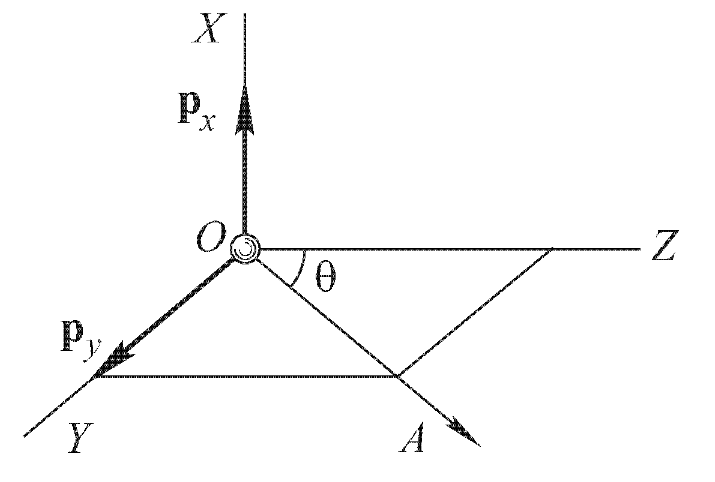
\includegraphics[width=0.25\textwidth]{figures/95_1.png}
    \caption{Рассеяние естественного света}
    \label{fig:freaky}
\end{figure}
Направим ось $X$ нормально к $OA$ и $OZ$, в силу $\vc{p} \parallel \vc{E}_0$ верно, что $\vc{p} \parallel XY$, тогда по найденному значению для $I_1$ с $\theta = \pi/2$ и $\theta = \pi/2- \vartheta$, можем найти интенсивности дипольных моментов $\vc{p}_x$ и $\vc{p}_y$. В силу ествественности падающего света, эти излучения \textit{некогерентны}, точнее некогерентны интенсивности от $\vc{p}_x$ и $\vc{p}_y$:
\begin{equation*}
    I_{1, \smallvc{p}_x} = 9 \varepsilon_0^2 \left(
        \frac{\varepsilon-\varepsilon_0}{\varepsilon+2 \varepsilon_0}
    \right)^2 \frac{\pi^2 V_1^2}{\lambda^4} \frac{\sin^2 \pi/2}{r^2} I_0,
    \hspace{10 mm} 
    I_{1, \smallvc{p}_y} = 9 \varepsilon_0^2 \left(
        \frac{\varepsilon-\varepsilon_0}{\varepsilon+2 \varepsilon_0}
    \right)^2 \frac{\pi^2 V_1^2}{\lambda^4} \frac{\cos^2 \vartheta}{r^2} I_0,
\end{equation*}
так что их можно просто сложить, тогда получим
\begin{equation*}
     I_1 
     =
    \frac{\omega^4}{4 \pi \varepsilon_0 v^3 r^2} \left(
        \overline{p_x^2} + \overline{p_y^2} \cos^2 \vartheta
     \right) 
     = 
     \frac{\omega^4}{4 \pi \varepsilon_0 v^3 r^2} \frac{1+\cos^2 \vartheta}{2} \overline{p^2} 
     =
     9 \varepsilon_0^2 \fbr{\varepsilon-\varepsilon_0}{\varepsilon+2 \varepsilon_0}^2 \frac{\pi^2 V_1^2}{\lambda^4} \frac{1+\cos^2 \theta}{2 r^2} I_0,
 \end{equation*} 
 где учтено $\overline{p_x^2} = \overline{p_y}^2 = \frac{1}{2} \overline{p^2}$. 
 а формула для $\mathcal P_1$ останется без изменений. 




\textbf{Частично поляризованный свет}. Полная линейная поляризация наблюдается только при $OA \bot $ направлению распространения падающего света, так как тогда $\vc{p}_y$ не даёт излучения. 


Если же посчитать интенсивность $I$ света, рассеиваемого объемом $V$, содержащим много шариков $\sub{N}{шар} V$, то, складывая интенсивности и рассматривая $r^3 \gg V$, найдём
\begin{equation*}
    I = 9 \varepsilon_0^2 \fbr{\varepsilon-\varepsilon_0}{\varepsilon+2 \varepsilon_0}^2
    \pi^2 \frac{V_1^2}{\lambda^4} \frac{1+\cos^2 \theta}{2 r^2} N V I_0.
\end{equation*}
Эта формула была получена Рэлеем, и по ней $I \sim \omega^{-4}$, что называют \textit{законом Рэлея}, что справедливо для сред с частицами, размеры которых малы по сравнению с длиной волны. 



\textbf{Убывание интенсивности}. Выделим цилиндр $\parallel OZ$ и рассмотрим баланс $I_0 (z) - I_0 (z+\d z) = \d I_0 = \mathcal P_1 N \d z$, тогда
\begin{equation*}
    \d I_0 = - \gamma I_0 \d z, \hspace{10 mm} 
    \gamma = 24 \pi^3 \varepsilon_0^2 \fbr{\varepsilon-\varepsilon_0}{\varepsilon+2 \varepsilon_0}^2 \frac{N V_1^2}{\lambda^4},
    \hspace{0.5cm} \Rightarrow \hspace{0.5cm}
    I_0 = \const \cdot e^{- \gamma z},
\end{equation*}
где $\gamma$ -- \textit{коэффициент рассеяния}.


\textbf{Молекулярное рассеяние (рассеяние Рэлея)}. 
Стоит заметить, что в атмосфере рассеяние происходит не посторонними частицами, а самими \textit{молекулами воздуха}. Такое рассеяние света называется \textit{рэлеевским} или \textit{молекулярным рассеянием}. На самом деле\footnote{
    1908 г., М. Смолуховский.
}  молекулярное рассеяние вызывается тепловым флуктуациями показателя преломления, которые и делают среду оптически мутной. 


Среда разбивается на $dV \ll \lambda^3$, при этом $N \d V \gg 1$. 
Уравнения на $\vc{H}'$ и $\vc{E}'$ остаются верны, последовательными приближениями можем получить
\begin{equation*}
    \delta \vc{P} = \frac{\delta \varepsilon}{4\pi} \vc{E}_0,
    \hspace{5 mm} 
    \vc{p} = \frac{\delta_i \varepsilon \cdot \delta_i V}{4 \pi} \vc{E}_0.
\end{equation*}
Это выражение отличается от случая с <<шариками>> только коэффициентом, так что верно, что
\begin{equation*}
    I_i = \frac{\pi^2}{\lambda^4} \frac{1 + \cos^2 \theta}{2 r^2} I_0 (\delta_i V)^2 \overline{(\delta_i \varepsilon)^2}.
\end{equation*}

Так, например, в случае идеального газа, верна формула
\begin{equation*}
    \varepsilon_i = 1 + 4 \pi \beta \frac{N_i}{\delta_i V},
\end{equation*}
где $\beta$ -- поляризуемость молекулы, а $N_i$ -- число молекул в $\delta_i V$. Так как $\delta_i V$ фиксирован, то $\delta_i \delta \varepsilon_i = 4 \pi \beta \delta N_i$, т.е. рассеяние вызывается \textit{флуктуациями числа молекл} в $\delta_i V$.


% см. 638 Сивухина
Аккуратно работая с этими флуктуациями, можем получить \textit{формулу Рэлея}:
\begin{equation*}
    I = \frac{2\pi^2}{\lambda^4} \frac{V}{N} (n-1)^2 \frac{1+\cos^2 \theta}{r^2} I_0,
\end{equation*}
что верно для изотропных молекул.


Для неидеальных газов и жидкостей можно получить формулу, вида
\begin{equation*}
    I = \frac{\pi^2}{\lambda^4} \frac{1+\cos^2 \theta}{2 r^2} V  I_0 \cdot
    \left(\rho \frac{d \varepsilon}{d \rho} \right)^2 \frac{kT}{(- v \partial_v P)_T},
\end{equation*}
полученную Эйнштейном в 1910 г. 

